\documentclass[UTF8]{beamer}

\usetheme{Madrid}
\usecolortheme{seagull}

\usepackage[english]{babel}
\usepackage{ctex}
\usepackage{algorithm,algorithmicx,algpseudocode}
\usepackage{tabularx}
\usepackage{graphicx}
\graphicspath{ {img/} }

\begin{document}

\title{Hush up! 题目讨论}
\author{CyanD1317 / Tommyr7 / wangyurzee}
\frame{\titlepage}


\begin{frame}{Problem 1. STUMBLER}

给定一个简化的物件组成的 osu! 谱面,从原点出发等概率选择一个方向发出一条射线,%
求有且仅有一个物件在射线上的概率。

\begin{itemize}
    \item $N_\mathrm{C}, N_\mathrm{S} \leq 50\,000$
    \item 精度 $10^{-6}$
\end{itemize}

\end{frame}

\begin{frame}{Observations \& Lemmata}

\begin{itemize}
\item
    将 $-\pi$ 和 $+\pi$ 看作首尾相接,那么一个物件影响的角度范围是连续的,%
    且该范围不会大于等于 $\pi$。
    \begin{itemize}
        \pause
        \item Formally:如果射线 $OA$ 与射线 $OB$ 都与物体 $U$ 有公共点,
            那么在劣角 $AOB$ 内的任意一条射线 $OC$ 都与物体 $U$ 有公共点。
        \pause
        \item 显然成立。
    \end{itemize}
\pause
\item
    在前两个子任务的限制下,物件影响的角度范围没有重叠部分。
    \begin{itemize}
        \pause
        \item 计算出每个物件的影响的范围大小,相加即为答案。
    \end{itemize}
\end{itemize}

\end{frame}

\begin{frame}{Algorithm 1}

子任务 1:只有圆形物件,物件影响的角度范围没有重叠部分。

\begin{figure}[h]\centering
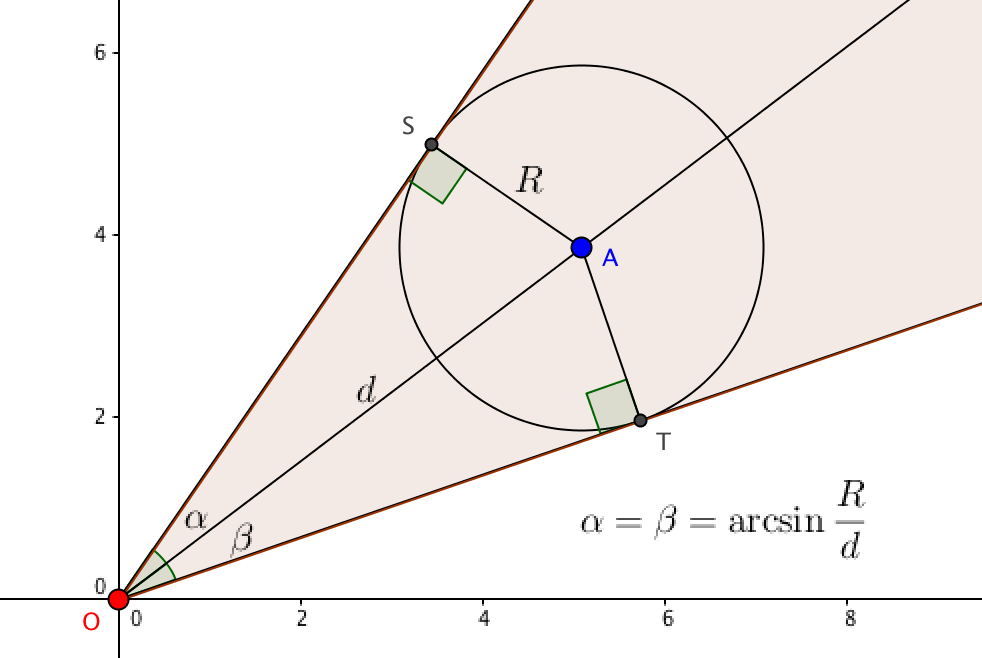
\includegraphics[scale=0.48]{a1.png}
\end{figure}

\end{frame}

\begin{frame}{Algorithm 2}

子任务 2:有滑条物件,物件影响的角度范围没有重叠部分。

\begin{figure}[h]\centering
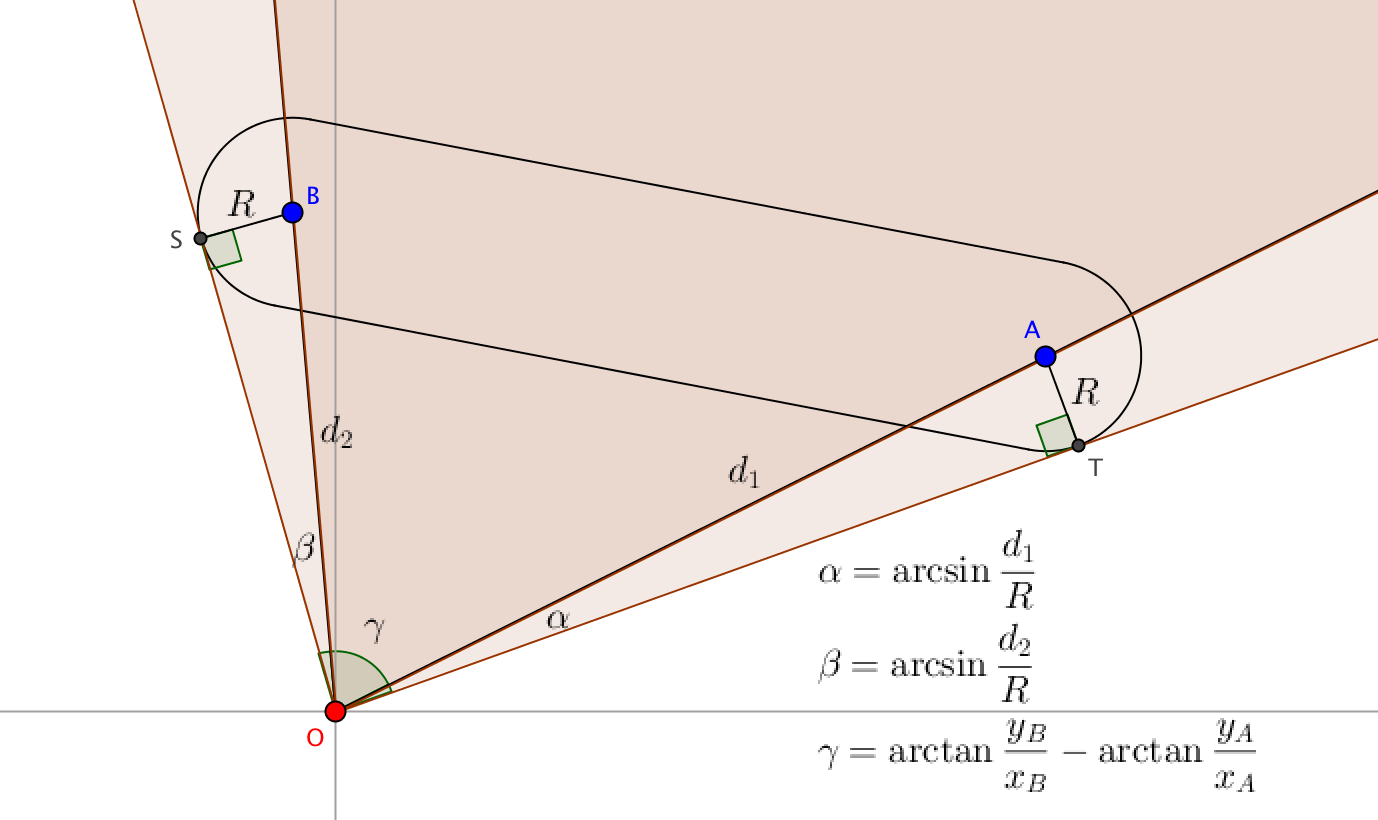
\includegraphics[scale=0.4]{a2.png}
\end{figure}

\end{frame}

\begin{frame}{Algorithm 2}

特殊情况:与上一种取 max

\begin{figure}[h]\centering
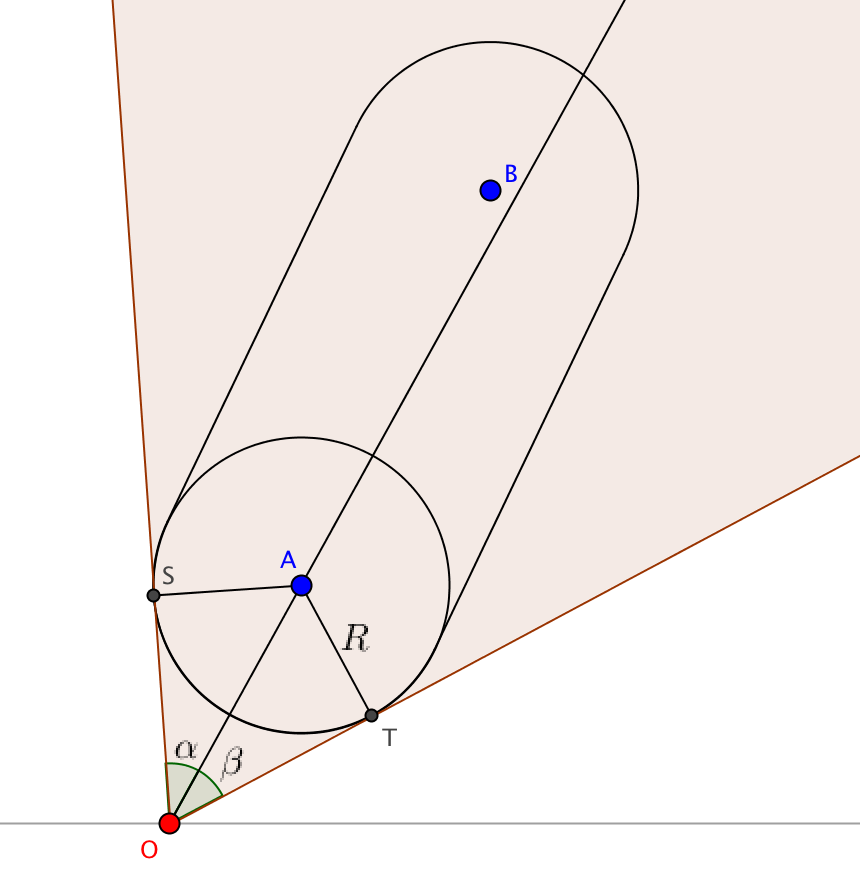
\includegraphics[scale=0.4]{a3.png}
\end{figure}

\end{frame}

\begin{frame}{Algorithm 3}

子任务 3:$N_\mathrm{C}, N_\mathrm{S} \leq 1\,000$ \newline

不会做,输出 QAQ

\begin{figure}[h]\centering

\includegraphics[scale=0.5]{xx.png}
\end{figure}

\end{frame}

\begin{frame}{Algorithm 4}

子任务 4:存在一条从原点出发的射线与每一个打击物件都有公共点。

\begin{figure}[h]\centering
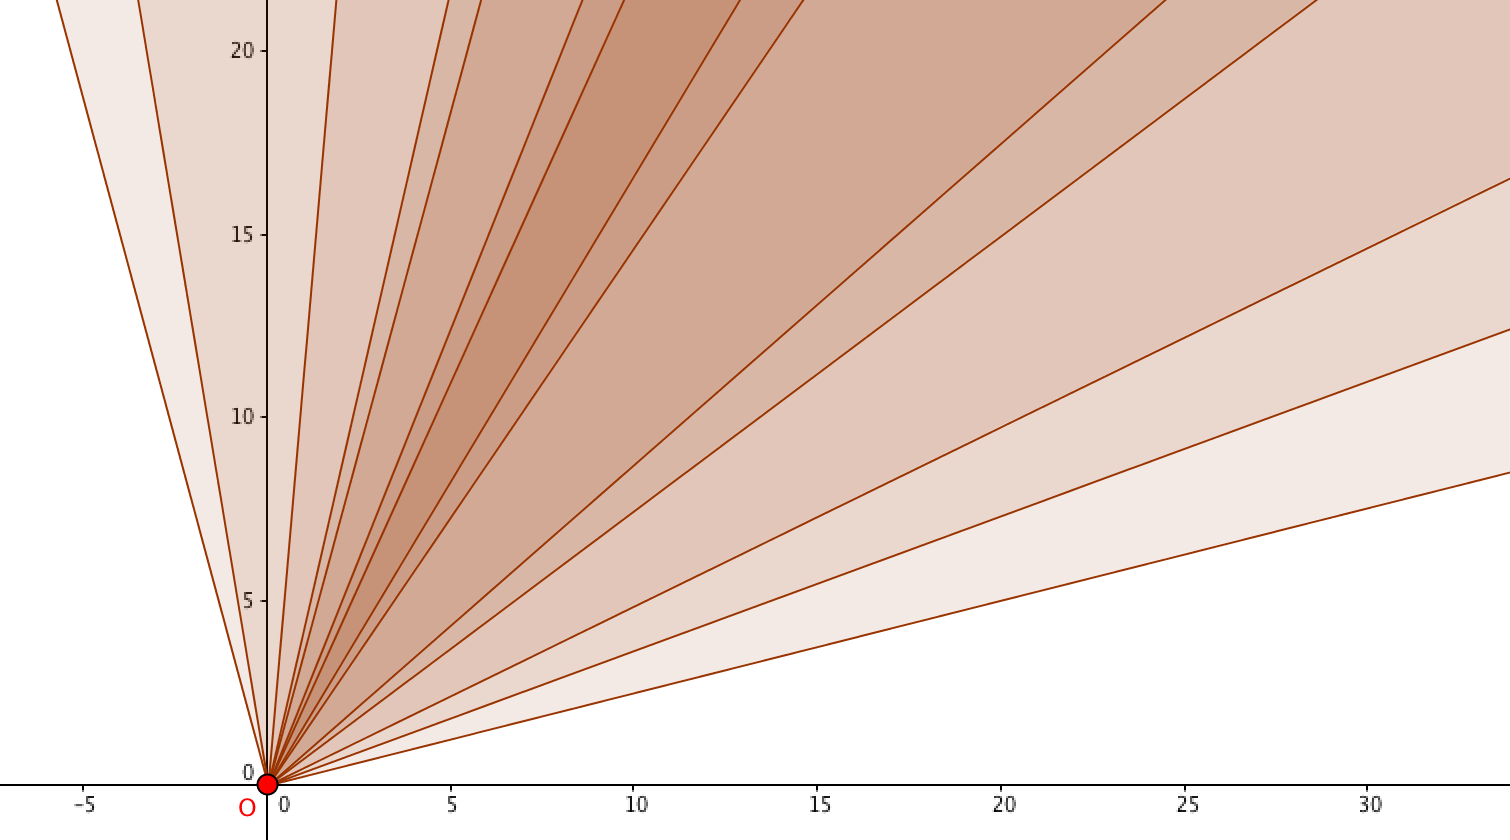
\includegraphics[scale=0.4]{a4.png}
\end{figure}



\end{frame}

\begin{frame}{Algorithm 5}

子任务 3:$N_\mathrm{C}, N_\mathrm{S} \leq 1\,000$ \newline

\begin{itemize}
    \pause \item 按照上述方法计算出每个物件影响角度的区间,记录端点(线?←\_←)并排序
    \pause \item 跨过 $\pm \pi$ 的位置拆分为两个区间
    \pause \item 枚举两个相邻端点,检查它们所夹区间是否被恰好一个物件覆盖
    \pause \item 排序 $O(N^2)$,枚举共 $O(N)$ 个区间,检查一次 $O(N)$
    \item 总时间复杂度 $O(N^2)$
\end{itemize}

\end{frame}

\begin{frame}{Algorithm 6}

我会快速排序!
\includegraphics[scale=0.666]{yy.png} \newline\newline

\pause $O(N \log N) + O(N^2) = O(N^2)$

\end{frame}

\begin{frame}{Algorithm 7}

“枚举两个相邻端点,检查它们所夹区间是否被恰好一个物件覆盖”\newline\newline

优化?

\end{frame}

\begin{frame}{Algorithm 7}

\begin{figure}[h]\centering
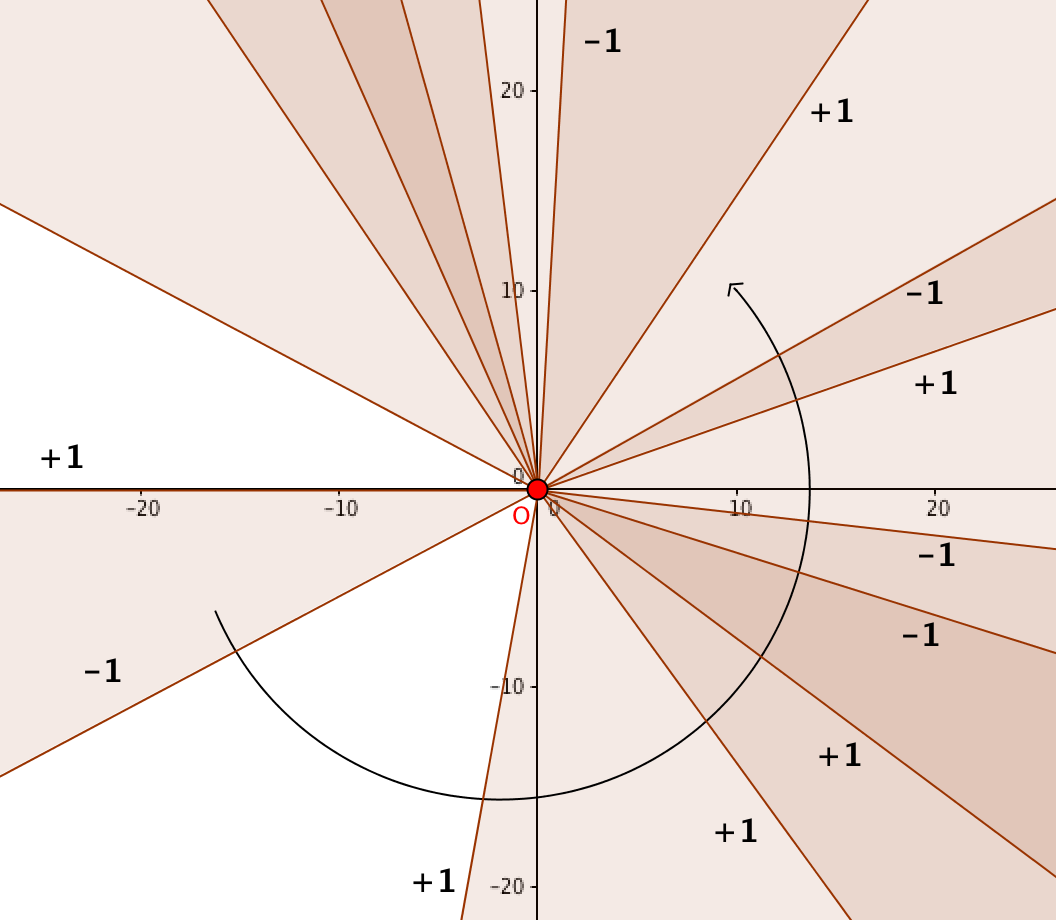
\includegraphics[scale=0.333]{a5.png}
\end{figure}

把区间转化成“事件”,对事件排序并依次处理,记录上个事件的位置与%
当前覆盖层数,判断层数 = 1 时增加答案。(常用 trick)

时间复杂度 $O(N \log N) + O(N) = O(N \log N)$

\end{frame}


\begin{frame}{Problem 2. OBSESSED}

给定一个序列,每个位置上为“空”、“面”音符与“边”音符中的一种。

进行下列操作:
\begin{itemize}
    \item 放置“面”或“边”音符;
    \item 询问一段连续区间内最近一对相同音符(“面”或“边”)之间的最小距离。
\end{itemize}

$N, M \leq 300\,000$

\end{frame}

\begin{frame}{Algorithm 1}

子任务 1、2:$N \cdot M \leq 600\,000$

直接模拟即可。注意反转操作的判定\newline\newline

\begin{algorithm}[H]
\begin{algorithmic}[1]
    \If {$A[i] = \mathrm{DON}$}
        \State $A[i] \gets \mathrm{KAT}$
    \Else
        \State $A[i] \gets \mathrm{DON}$
    \EndIf
\end{algorithmic}
\caption{ 
\includegraphics[scale=0.2]{zz.jpg}}
\label{alg:seq}
\end{algorithm}

\end{frame}

\begin{frame}{Algorithm 2}

子任务 3:没有“边”音符和反转操作,放置音符的位置严格单调递增

\begin{figure}[h]\centering
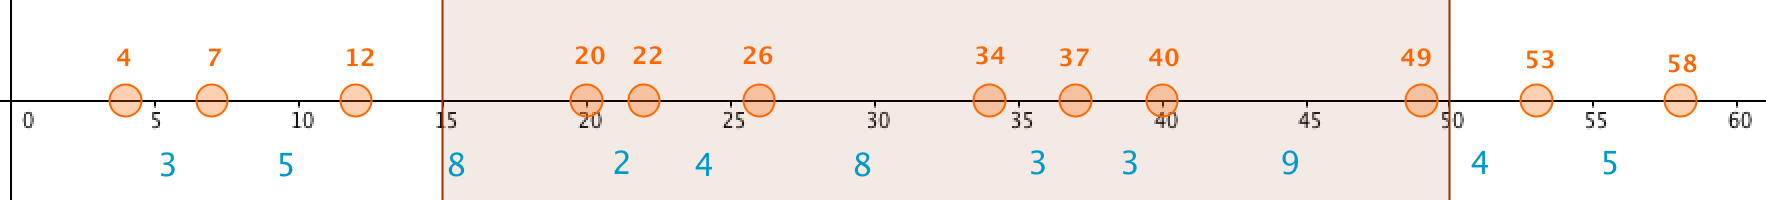
\includegraphics[scale=0.4]{b1.png}
\end{figure}

\begin{itemize}
    \pause \item 找出对应的音符范围:二分查找,$O(\log N)$
    \pause \item 在范围内查询最小值:Range Minimum Query,线段树 $O(\log N)$
\end{itemize}

\end{frame}

\begin{frame}{Algorithm 3}

子任务 4:存在两种音符,没有反转操作 \newline\newline

看着好像线段树的样子

\end{frame}

\begin{frame}{Algorithm 3}

对于一个线段树的节点而言,需要考虑的情况有以下三种:
\begin{itemize}
    \item 完全在左子节点的区间中;
    \item 完全在右子节点的区间中;
    \item 跨越左右子节点区间的交界处。
\end{itemize}

\pause
为了实现两段区间信息的合并,需要在每个节点上记录……?

\pause
\textbf{最左/最右的鼓面/鼓边音符}共 4 条信息。\\
另外自己内部的最优答案也要记录。

\end{frame}

\begin{frame}{Updating Segment Tree Nodes}

\begin{algorithm}[H]
\begin{algorithmic}[1]
    \Function {Update}{$node$}
        \If {$node.lch = -1$} \State \Return \EndIf
        \State $node.lmost\_don = \min(node.lch.lmost\_don, node.rch.lmost\_don)$
        \State $node.rmost\_don = \min(node.lch.rmost\_don, node.rch.rmost\_don)$
        \State $node.lmost\_kat = \min(node.lch.lmost\_don, node.rch.lmost\_kat)$
        \State $node.rmost\_kat = \min(node.lch.rmost\_don, node.rch.rmost\_kat)$
        \State $node.ans = \min(node.lch.ans, node.rch.ans)$
        \State $node.ans = \min(node.ans, node.rch.lmost\_don - node.lch.rmost\_don)$
        \State $node.ans = \min(node.ans, node.rch.lmost\_kat - node.lch.rmost\_kat)$
    \EndFunction
\end{algorithmic}
\caption{}
\label{alg:seq}
\end{algorithm}

\end{frame}

\begin{frame}{Algorithm 3}

时间复杂度 $O(M \log N)$。

\end{frame}

\begin{frame}{Algorithm 4}

子任务 5:存在两种音符和反转操作 \newline\newline

看着好像线段树的样子

\begin{figure}[h]\centering

\includegraphics[scale=0.5]{xx.png}
\end{figure}

\end{frame}

\begin{frame}{Algorithm 4}

\textbf{延迟标记/懒标记}

每个节点除了记录上述信息外,额外记录一个布尔变量 $tag$%
表示该节点下所有的音符是否被 Invert

维持 $lmost, rmost$ 与 $tag$ 同步更新(即 $lmost, rmost$%
记录的是 $tag$ 生效后的值)。访问到一个节点时,若该节点的%
$tag$ 为真,那么将 $tag$ 下传到左右子节点并更新各自信息。

\end{frame}

\begin{frame}{Handling Lazy Tag Propagation}

\begin{algorithm}[H]
\begin{algorithmic}[1]
    \Function {PushDown}{$node$}
        \If {$node.lch = -1$ \textbf{or} $node.tag = $ \textbf{false}}
            \State \Return
        \EndIf
        \State $node.tag \gets$ \textbf{false}
        \State $node.lch.tag \gets$ \textbf{not} $node.lch.tag$
        \State $node.rch.tag \gets$ \textbf{not} $node.rch.tag$
        \State \Call{Swap}{$node.lch.lmost\_don, node.lch.lmost\_kat$}
        \State \Call{Swap}{$node.lch.rmost\_don, node.lch.rmost\_kat$}
        \State \Call{Swap}{$node.rch.lmost\_don, node.rch.lmost\_kat$}
        \State \Call{Swap}{$node.rch.rmost\_don, node.rch.rmost\_kat$}
    \EndFunction
\end{algorithmic}
\caption{}
\label{alg:seq}
\end{algorithm}

\end{frame}

\begin{frame}{Algorithm 4}

时间复杂度 $O(M \log N)$。

具体细节参见参考程序或者两段伪代码。

\end{frame}

\begin{frame}{Problem 3. CACCEPT}

\xout{(其实这就是上学期期末的 Hako 窝怎么会说呢)} \newline\newline

交互题。有一个五个不同字母的排列,每次可以询问五个字母(可以重复),得到:
\begin{itemize}
    \item 有多少个在答案中位置正确的字母;
    \item 有多少个不同的在答案中出现但位置不正确的字母。
\end{itemize}

用最少的询问次数确定字母排列。按照谜之公式给分。

\pause
评分参数 $L = 11$ \xout{知道泥萌很好奇}

\end{frame}

\begin{frame}{Algorithm 1}

直接提交样例程序,可以卡着时限通过所有 20 组数据。

平均每组数据需要花费上千万次询问,效率得分 $E \approx 0$。\newline\newline

\pause 期望得分 20 分。

\end{frame}

\begin{frame}{Algorithm 2 by wangyurzee}

从“ABCDE”(随机亦可)开始尝试对于每一位进行调整,保留返回值最大的答案。\newline\newline

\pause 最大单次尝试次数 $5 \times 26 = 130$,实际最大单次 116、合计 2320,
期望得分 25 \textasciitilde 30 分。

\end{frame}

\begin{frame}{Algorithm 3 by wangyurzee}

在算法二的基础上进行特别判断,如果一次调整将返回值增加了 9(完全猜对了一位)%
那么退出当前位的调整进入下一位。\newline\newline

\pause 最大单次尝试次数仍为 130,实际最大单次 94、合计 1236,
期望得分 30 \textasciitilde 40 分。

\end{frame}

\begin{frame}{Algorithm 4}

从 A 到 Z 分别重复五遍进行询问(“AAAAA”、“BBBBB”……)找出所有出现的的字母。

枚举五个字母的排列并逐次询问。\newline\newline

\pause 最大单次尝试次数 $26 + 5! = 146$,期望得分 25 \textasciitilde 35 分。

\end{frame}

\begin{frame}{Algorithm 5}

在算法四的基础上,不枚举排列而是枚举 $\binom{5}{2} = 20$ 对元素%
并尝试交换,保留返回值大的答案。\newline\newline

\pause 最大单次尝试次数 $26 + \binom{5}{2} = 46$,实际最大单次 37、合计 740,
期望得分 40 \textasciitilde 50 分。

\end{frame}

\begin{frame}{Algorithm 6 by wangyurzee}

在算法五的基础上改进第一部分的找字母过程。

\pause 每次进行形如“ABABA”的询问,其中含有的字母个数有三种情况:
\begin{itemize}
    \item 0:直接确定 A、B 均不在答案内出现;
    \item 2:直接确定 A、B 均在答案内出现;
    \item 1:进行另一次询问“AAAAA”,确定是 A 还是 B 在答案内出现。
\end{itemize} 

\pause 最大单次尝试次数 $\frac{26}{2} + 5 + \binom{5}{2} = 38$,实际最大单次 29、合计 509,
期望得分 50 \textasciitilde 55 分。

\end{frame}

\begin{frame}{吐槽时间}
\end{frame}

\begin{frame}{Algorithm 7}

首先我们需要知道 $L = 11$ 是哪里来的……

\pause (知道了不就会做了?
\pause (并不

\end{frame}

\begin{frame}{Entropy}

\xout{以下内容均为口胡}

在信息论中,熵是接收的每条消息中包含的信息的平均量,%
可以理解为不确定性的量度。

简单的解释:有 $N$ 个互斥事件,其中第 $i$ 个事件 $x_i$ 发生的概率为 $P(x_i)$,
且它们是 collectively exhaustive events 即 $\sum P(x_i) = 1$,那么该体系的熵等于

$$
    H(X) = -\sum_{i} P(x_i) \log_2 P(x_i)
$$

例如抛一枚硬币事件的熵为 1(提供了 1 bit 的信息),%
掷一次骰子事件的熵为 $-6 \cdot \frac{1}{6} \log_2 \frac{1}{6} \approx 2.6$。

\end{frame}

\begin{frame}{Entropy}

$$
    H(X) = -\sum_{i} P(x_i) \log_2 P(x_i)
$$

\begin{itemize}
    \item \xout{萌萌哒的}华二气象台认为某天的降水概率是 50\%,当天下雨
    \item \xout{萌萌哒的}华二气象台认为某天的降水概率是 99.99\%,当天下雨
\end{itemize}

\pause
第一种情况:降水这一事件提供了 $1$ bit 信息\\
第二种情况:降水这一事件提供了 $1.47 \times 10^{-3}$ bit 信息 \newline\newline

信息来源的熵越大,一条消息包含的信息量也就越大。

\end{frame}

\begin{frame}{Entropy}

在假设每个文字出现在文本中的概率相同的情况下:
\begin{itemize}
    \item 英文字母的熵约为 4.7(实际占用 8 bits,58.8\%)
    \item 日文平假名的熵约为 5.64(实际占用 8 bits,70.5\%)
    \item 汉字的熵约为 11.3(实际占用 16 bits,70.6\%)
\end{itemize}
\pause
\begin{figure}[h]\centering

\includegraphics[scale=0.028]{uu.jpg}
\end{figure}

\end{frame}

\begin{frame}{Algorithm 7}

回到本题,一次询问的结果有 00、01、……、40、41、50 共 21 种。

\pause
第一次询问时可以将答案视为随机,因此每个结果发生的概率 = %
所有五字母的排列中能产生该结果的排列数量/所有这样的排列数量。

\pause
可以得到,第一次询问作为一个信息源,它的熵大约为 2.289。%
也就是说,第一次询问可以得到 2.289 bits 的信息。

事(cai)实(ce)上如果采取最优策略,每一次询问包含的信息量都可以达到 2 bits 左右。

\pause
确定一个五个不重复字母的排列需要至少 %
$\log_{2} 26 \times 25 \times 24 \times 23 \times 22 \approx 22.912$ %
bits 的信息量。因此其理论下界 $L = \left\lfloor \frac{22.9125}{2.289} \right\rfloor = 11$。

\end{frame}

\begin{frame}{Algorithm 7}

\begin{figure}[h]\centering

\includegraphics[scale=0.5]{vv.jpg}
\end{figure}

然而这道题还是不会做……

\end{frame}

\begin{frame}{Algorithm 7}

知道了下界 11 之后,我们可以枚举每一步的询问,%
构造出一棵 $(26^5 \times 21)^{11}$ 个节点的树,询问的时候按照答案在上面一步一步走,%
选择最小的子树进行下一步询问(这样能保证尽快到达叶子节点找到解)就可以了(正经脸 \newline\newline

\pause 期望得分 0 分。

\end{frame}

\begin{frame}{Algorithm 8}

既然样本空间辣么大,随机化应该可以达到不错的效果!

\pause
建树神马的太麻烦……

维护一个列表,保存满足之前所有询问结果的可能的排列。%
每次询问过后,扫描列表,去除不满足本次询问结果的元素。

\pause
随机选择 $C$ 个五个字母的排列作为下一次询问的候选。%
对于每个候选,随机从上述列表中选择 $T$ 个,在该候选询问上得到结果,%
并以此近似计算出该询问带来的信息量。

选择 $C$ 个候选中信息量最大的进行询问即可。

\pause
实现时该列表直接采用数组,取 $C = 4096, T = 768$。在这个数量级上的 %
$C$ 和 $T$ 值都能在时限内达到很好的成绩。

\end{frame}

\begin{frame}{Algorithm 8}

最坏情况未知,期望单组数据尝试次数约为 12。

实际尝试不同随机种子之后能够做到最大单组数据 11 次询问。

\pause
std 都有几率不拿蟒分,所以是 Challenge Accepted 啊……

\begin{figure}[h]\centering

\includegraphics[scale=0.5]{zz.jpg}
\end{figure}

(其实原来这题的中文名的想法是「挑战不可能」……)

\end{frame}

\begin{frame}{Acknowledgements}

感谢\xout{跳票的}验题菌 Tommyr7 和 wangyurzee。

感谢 arcGravitus、某菜鸡和 TkskKurumi(被)提供名字。

题目描述中所有电子设备均为虚构,如有雷同,请务必给我来一台。

感谢金老师和 CZR 的鼎力滋瓷,以及感谢大家能来做这次\xout{没啥区分度的偏}题。

\end{frame}

\end{document}

